%-------------------------------------------------------------------------------
%                                PREAMBLE
%-------------------------------------------------------------------------------
\documentclass[usenames,dvipsnames,svgnames,10pt,aspectratio=169]{beamer}
\usefonttheme{professionalfonts}

% This theme uses TIKZ: compile twice with PDFLaTeX or LuaLaTeX.
%
%  Options:
%  - [clean]:    clean slides, i.e. logos and footbar are removed
%  - [kth]:      footbar style inspierd to the official KTH template
%  - [nicewave]: a different style of wave is used (not approved by FLOW)
%
\usetheme{flow}

\usepackage{hyperref,graphicx,lmodern}
\usepackage[utf8]{inputenc}
\usepackage{media9}
\usepackage{xcolor}
\usepackage{stmaryrd}
\usepackage{nicefrac}
\usepackage{multimedia}
\usepackage{multicol}
\usepackage{upgreek}
\usepackage[]{bm}
\usepackage[]{url}

\DeclareMathOperator{\sinc}{sinc}
\DeclareMathAlphabet{\mathcal}{OMS}{cmsy}{m}{n}
\DeclareMathAlphabet\mathbfcal{OMS}{cmsy}{b}{n}
\DeclareMathOperator*{\minimize}{minimize~}
\DeclareMathOperator*{\subjectto}{subject~to~}

\graphicspath{{imgs/}}
\setbeamertemplate{blocks}[rounded][shadow=true]

\DeclareMathOperator{\trace}{tr}

%-------------------------------------------------------------------------------
%                                TITLE PAGE
%-------------------------------------------------------------------------------
\title[Nonlinear Physics] % Short title used in footline
{
	Nonlinear physics, dynamical \\ systems and chaos theory
}

\author[J.-Ch.~Loiseau] % Presenting author in short form used in footline
{
	Jean-Christophe Loiseau
}
% - Give the names in the same order as the appear in the paper.
% - Underline the presenting author.

\institute[unused]
{
	\url{jean-christophe.loiseau@ensam.eu} \\
	DynFluid, \\
	Arts et M\'etiers ParisTech, France
}
% Keep it simple, no one is interested in your street address.

% University logo(s)
\logot{\includegraphics[width=.128\paperwidth]{DynFluid_logo}}  % Top logo
\logob{\includegraphics[width=0.128\paperwidth]{ENSAM_logo}} % Bottom logo
% \logoc[{\includegraphics[width=.128\paperwidth]{limsi}}]{\includegraphics[width=.128\paperwidth]{limsi}} % Corner logo
%
% Cover image: \cvrimg{x position}{y position}{cover image}
\cvrimg{.77}{.8}{\includegraphics[width=.4\paperwidth]{cover.png}}

\date[unused]{ENSAM, Master 2, 2018--2019}

\begin{document}

\titleframe % Print the title as the first slide

%-------------------------------------------------------------------------------
%                           PRESENTATION SLIDES
%-------------------------------------------------------------------------------

\begin{frame}[t, c]{Today's menu}{Dimensionality reduction}
	\centering
	\begin{columns}
		\begin{column}{.33\textwidth}
			\centering
			\includegraphics[width=\columnwidth]{dimensionality_reduction}
		\end{column}
		\begin{column}{.4\textwidth}
			\centering
			\includegraphics[width=\columnwidth]{svd}
		\end{column}
	\end{columns}

	\bigskip

	\begin{tabular}{ll}
		\textbf{Examples:} & Fourier Mode Decomposition, Proper Orthogonal Decomposition (POD), \\
		~                  & Dynamic and Koopman Mode Decomposition (DMD), Resolvent modes, ...
	\end{tabular}

	\vspace{1cm}
\end{frame}

\begin{frame}[t, c]{}
	\centering
	\vspace{1cm}

	{\Large \textbf{Singular Value Decomposition}}

	\bigskip

	{\textgre{\textbf{One of the big six matrix decompositions}}}

\end{frame}

\begin{frame}[t, c]{Matrix decomposition}{The big six}
	Stewart (\emph{Comput. Sci. Engrg.}, \textbf{2}: 50-59, 2000) has list the \emph{big six matrix decompositions}:
	\begin{enumerate}
		\item Cholesky decomposition
		\item pivoted LU decomposition
		\item QR decomposition
		\item Spectral decomposition
		\item Schur decomposition
		\item \alert{\textbf{Singular Value Decomposition}}
	\end{enumerate}
	\vspace{1cm}
\end{frame}

\begin{frame}[t, c]{Singular Value Decomposition}{Definition}
	\begin{minipage}{.48\textwidth}
		Given $\mathbfcal{A} \in \mathbb{C}^{m \times n}$, there exists a factoratization of $\mathbfcal{A}$ such that
		$$\mathbfcal{A} = \mathbfcal{U} \boldsymbol{\Upsigma}\mathbfcal{V}^H$$
		where
		\begin{itemize}
			\item $\mathbfcal{U}$ is a $m \times m$ \emph{unitary} matrix, i.e.\ $\mathbfcal{U}^H \mathbfcal{U} = \mathbfcal{I}$.
			\item $\boldsymbol{\Upsigma}$ is a \emph{diagonal} $m \times m$ matrix with non-negative real numbers $\sigma$ on the diagonal.
			\item $\mathbfcal{V}^H$ is a $n \times n$ \emph{unitary} matrix.
		\end{itemize}
	\end{minipage}%
	\hfill
	\begin{minipage}{.48\textwidth}
		\centering
		\includegraphics[width=.9\textwidth]{svd}
	\end{minipage}

	\vspace{1cm}
\end{frame}

\begin{frame}[t, c]{Singular Value Decomposition}{Definition}
	\begin{itemize}
		\item The first $p = \min(m, n)$ columns of $\mathbfcal{U}$ and $\mathbfcal{V}$ are known as the \emph{left} and \emph{right} singular vectors of the matrix $\mathbfcal{A}$.

		\bigskip

		\item They are related by
		$$\mathbfcal{A} \mathbf{v}_i = \sigma_i \mathbf{u}_i$$
		and
		$$\mathbfcal{A}^H \mathbf{u}_i = \sigma_i \mathbf{v}_i.$$
	\end{itemize}

	\vspace{1cm}
\end{frame}

\begin{frame}[t, c]{Singular Value Decomposition}{Properties}
	Let us assume that $\mathbfcal{U}$, $\boldsymbol{\Upsigma}$ and $\mathbfcal{V}$ are block-partitioned such that

	\begin{center}
		\begin{tabular}{ccc}
			$\mathbfcal{U} = \begin{bmatrix} \mathbfcal{U}_1 & \mathbfcal{U}_2 \end{bmatrix}$ & $\boldsymbol{\Upsigma} = \begin{bmatrix} \boldsymbol{\Upsigma}_1 & 0 \\ 0 & \boldsymbol{\Upsigma}_2 \end{bmatrix}$ & $\mathbfcal{V} = \begin{bmatrix} \mathbfcal{V}_1 & \mathbfcal{V}_2 \end{bmatrix}$
		\end{tabular}
	\end{center}
	with
	\begin{center}
		\begin{tabular}{cc}
			$\boldsymbol{\Upsigma}_1 = \begin{bmatrix} \sigma_1 & ~ & ~ \\ ~ & \ddots & ~ \\ ~ & ~ & \sigma_r \end{bmatrix}$ & $\boldsymbol{\Upsigma}_2 = 0 \in \mathbb{R}^{(m-r) \times (n-r)}$
		\end{tabular}
	\end{center}

	\vspace{1cm}
\end{frame}

\begin{frame}[t, c]{Singular Value Decomposition}{Properties}
	\begin{itemize}
		\item One can easily show that
		\begin{itemize}
			\item[$\hookrightarrow$] Rank $\mathbfcal{A} = r$,
			\item[$\hookrightarrow$] Dyadic decomposition: $\mathbfcal{A} = \sum \limits_{i=1}^{r} \sigma_i \mathbf{u}_i \mathbf{v}_i^H$
			\item[$\hookrightarrow$] The Frobenius norm $\| \mathbfcal{A} \|_F^2 = \sum \limits_{i=1}^r \sigma_i^2$
		\end{itemize}

		\bigskip

		\item It moreover has connections with eigenvalue decomposition:
		\begin{center}
			\begin{tabular}{cc}
				$\mathbfcal{A}^H \mathbfcal{A} = \mathbfcal{V} \boldsymbol{\Upsigma}^2 \mathbfcal{V}^H$ & $\mathbfcal{A} \mathbfcal{A}^H = \mathbfcal{U} \boldsymbol{\Upsigma}^2 \mathbfcal{U}^H$
			\end{tabular}
		\end{center}
	\end{itemize}

	\vspace{1cm}
\end{frame}

\begin{frame}[t, c]{Singular Value Decomposition}{Applications}
	\begin{itemize}
		\item SVD is used in a broad range of applications:
		\begin{itemize}
			\item[$\hookrightarrow$] Data compression,
			\item[$\hookrightarrow$] Computation of the Moore-Penrose pseudo-inverse,
			\item[$\hookrightarrow$] Solving $\mathbfcal{A} \mathbf{x} = \mathbf{0}$,
			\item[$\hookrightarrow$] Low-rank matrix approximation,
			\item[$\hookrightarrow$] Statistics,
			\item[$\hookrightarrow$] ...
		\end{itemize}

		\bigskip

		\item In the rest of this course, we will use it to extract so-called \emph{coherent structures} from a large-scale dataset.
	\end{itemize}

	\vspace{1cm}
\end{frame}

\begin{frame}[t, c]{Singular Value Decomposition}{Example: low-rank approximation}
	\begin{itemize}
		\item The low-rank approximation problem reads
		\begin{equation}
			\begin{aligned}
				& \minimize_{\hat{\mathbfcal{A}}} = \| \mathbfcal{A} - \hat{\mathbfcal{A}} \|_F^2 \\
				& \subjectto \text{rank } \hat{\mathbfcal{A}} \leq r.
			\end{aligned}
			\notag
		\end{equation}

		\bigskip

		\item The solution to this minimization problem is given by the truncated SVD of $\mathbfcal{A}$, i.e.\
		$$\hat{\mathbfcal{A}} = \mathbfcal{U}_{1:r} \boldsymbol{\Upsigma}_{1:r} \mathbfcal{V}^H_{1:r}.$$

		\bigskip

		\item By choosing an appropriate $r$, one can control the error made by the low-rank approximation, that is
		$$\| \mathbfcal{A} - \hat{\mathbfcal{A}} \|_F^2 = \sigma^2_{r+1} + \cdots + \sigma_n^2.$$
	\end{itemize}

	\vspace{1cm}
\end{frame}

\begin{frame}[t, c]{}
	\centering
	\vspace{1cm}

	{\Large \textbf{Dimensionality Reduction: POD}}

	\bigskip

	{\textgre{\textbf{Extracting an optimal low-dimensional representation}}}

\end{frame}

\begin{frame}[t, c]{Proper Orthogonal Decomposition}{Other names}
	Proper Orthogonal Decomposition is also known as:
	\begin{itemize}
		\item Principal Component Analysis (PCA) is in statistical analysis,
		\item Kosambi-Karhunen-Loève transform (KLT) in signal processing,
		\item Empircal Orthogonal Function (EOF) in meteorological science,
		\item ...
	\end{itemize}

	\vspace{1cm}
\end{frame}

\begin{frame}[t, c]{Proper Orthogonal Decomposition}{Objectives}
	\begin{itemize}
		\item Let us consider an ensemble of snapshots of the time-evolution of our system
		$$\mathbfcal{Q} = \begin{bmatrix} \mathbf{q}(\bm{x}, t_1) & \mathbf{q}(\bm{x}, t_2) & \cdots & \mathbf{q}(\bm{x}, t_k) \end{bmatrix},$$
		so that $\mathbfcal{Q} \in \mathbb{C}^{n \times k}$.

		\bigskip

		\item The aim of POD analysis is to find a set of (spatial) structures that provide an optimal low-rank approximation of the data matrix $\mathbfcal{Q}$.
		\begin{itemize}
			\item[$\hookrightarrow$] This is clearly connected to the SVD of $\mathbfcal{Q}$!
		\end{itemize}
	\end{itemize}

	\vspace{1cm}
\end{frame}

\begin{frame}[t, c]{Proper Orthogonal Decomposition}{Illustration}
	\centering
	\begin{columns}
		\begin{column}{.33\textwidth}
			\centering
			\includegraphics[width=\columnwidth]{dimensionality_reduction}
		\end{column}
		\begin{column}{.4\textwidth}
			\centering
			\includegraphics[width=\columnwidth]{svd}
		\end{column}
	\end{columns}

	\vspace{1cm}
\end{frame}

\begin{frame}[t, c]{Proper Orthogonal Decomposition}{Temporal covariance}
	\begin{itemize}
		\item Let us define the temporal covariance between $\mathbf{q}_i$ and $\mathbf{q}_j$ as
		$$c_{ij} = \mathbf{q}_j^T \mathbfcal{M} \mathbf{q}_i,$$
		where $\mathbfcal{M}$ is a symmetric positive semi-definite matrix defining a physically meaningful inner product.

		\bigskip

		\item The complete matrix of temporal covariance is simply given by
		$$\mathbfcal{C} = \mathbfcal{Q}^T \mathbfcal{M} \mathbfcal{Q}.$$
	\end{itemize}

	\vspace{1cm}
\end{frame}

\begin{frame}[t, c]{Proper Orthogonal Decomposition}{Temporal covariance}
	\begin{minipage}{.48\textwidth}
		\begin{itemize}
			\item $c_{ij}$ characterizes how similar two snapshots $\mathbf{q}_i$ and $\mathbf{q}_j$ are.

			\bigskip

			\item $\mathbfcal{C}$ provides a visual representation of these similarities across the different $t_k$ considered.

			\bigskip

			\item Spectral decomposition of $\mathbfcal{C}$ informs us about the number of "active" degrees of freedom in the system.
		\end{itemize}
	\end{minipage}%
	\hfill
	\begin{minipage}{.48\textwidth}
		\centering
		\includegraphics[width=.66\textwidth]{kuramoto_sivashinky_temporal_correlation}

		{\small Temporal correlation matrix of a chaotic spatio-temporal system.}
	\end{minipage}

	\vspace{1cm}
\end{frame}

\begin{frame}[t, c]{Proper Orthogonal Decomposition}{Temporal covariance}
	\begin{minipage}{.48\textwidth}
		\begin{itemize}
			\item $c_{ij}$ characterizes how similar two snapshots $\mathbf{q}_i$ and $\mathbf{q}_j$ are.

			\bigskip

			\item $\mathbfcal{C}$ provides a visual representation of these similarities across the different $t_k$ considered.

			\bigskip

			\item Spectral decomposition of $\mathbfcal{C}$ informs us about the number of "active" degrees of freedom in the system.
		\end{itemize}
	\end{minipage}%
	\hfill
	\begin{minipage}{.48\textwidth}
		\centering
		\includegraphics[width=.66\textwidth]{shear_driven_cavity_covariance_matrix_zoom}

		{\small Temporal correlation matrix of a (almost) periodic spatio-temporal system.}
	\end{minipage}

	\vspace{1cm}
\end{frame}

\begin{frame}[t, c]{Proper Orthogonal Decomposition}{Eigenpairs of $\mathbfcal{C}$}
	\begin{minipage}{.48\textwidth}
		\begin{itemize}
			\item Spectral decomposition of $\mathbfcal{C}$ reads
			$$\mathbfcal{C} \mathbfcal{V} = \mathbfcal{V} \boldsymbol{\Uplambda}.$$

			\bigskip

			\item $\lambda_i$ characterizes how much variance is captured by the i\textsuperscript{th} eigenvector $\mathbf{v}_i$.

			\bigskip

			\item The leading eigenvectors $\mathbfcal{V}_{1:r}$ provide a low-dimensional representation of the original system explaining most of its variability.
		\end{itemize}
	\end{minipage}%
	\begin{minipage}{.48\textwidth}
		\centering
		\includegraphics[width=.66\textwidth]{kuramoto_sivashinky_temporal_correlation_eigenvalues}

		{\small Eigenvalues of $\mathbfcal{C}$ for the chaotic spatio-temporal system.}
	\end{minipage}

	\vspace{1cm}
\end{frame}

\begin{frame}[t, c]{Proper Orthogonal Decomposition}{Eigenpairs of $\mathbfcal{C}$}
	\begin{minipage}{.48\textwidth}
		\begin{itemize}
			\item Spectral decomposition of $\mathbfcal{C}$ reads
			$$\mathbfcal{C} \mathbfcal{V} = \mathbfcal{V} \boldsymbol{\Uplambda}.$$

			\bigskip

			\item $\lambda_i$ characterizes how much variance is captured by the i\textsuperscript{th} eigenvector $\mathbf{v}_i$.

			\bigskip

			\item The leading eigenvectors $\mathbfcal{V}_{1:r}$ provide a low-dimensional representation of the original system explaining most of its variability.
		\end{itemize}
	\end{minipage}%
	\begin{minipage}{.48\textwidth}
		\centering
		\includegraphics[width=.75\textwidth]{explained_variance_plot}

		{\small Eigenvalues of $\mathbfcal{C}$ for the (almost) periodic spatio-temporal system.}
	\end{minipage}

	\vspace{1cm}
\end{frame}

\begin{frame}[t, c]{Proper Orthogonal Decomposition}{Statistics}
	\begin{itemize}
		\item $\mathbfcal{C}$ is a symmetric positive-definite matrix, hence
		$$\mathbf{v}_i^T \mathbf{v}_j = \delta_{ij}.$$

		\medskip

		\item From a statistical point of view, POD thus extract \alert{\textbf{linearly uncorrelated}} coherent structures from the data.

		\bigskip

		\item One needs to be very careful when applying POD to a nonlinear system!
		$$\text{Linear uncorrelated}\quad \neq \quad \text{Nonlinearly uncorrelated}$$
	\end{itemize}

	\vspace{1cm}
\end{frame}

\begin{frame}[t, c]{Proper Orthogonal Decomposition}{Extracting the spatial structures}
	\begin{itemize}
		\item The spatial structure associated to the eigenpairs of $\mathbfcal{C}$ are given by
		$$\mathbfcal{U} = \mathbfcal{Q} \mathbfcal{V}.$$

		\bigskip

		\item These are known as the \alert{\textbf{POD modes}}. They provide an optimal projection basis to obtain a low-dimensional representation of the original system.
	\end{itemize}

	\vspace{1cm}
\end{frame}

\begin{frame}[t, c]{Proper Orthogonal Decomposition}{\underline{Illustration}: Shear-driven cavity flow}
	\begin{columns}
		\begin{column}{.45\textwidth}
			\begin{center}
				\includegraphics[width=\textwidth]{shear-driven-cavity}
			\end{center}
			\textbf{Figure:} Instantaneous vorticity colormap at $Re=7500$ (based on cavity's depth).
		\end{column}
		\begin{column}{.55\textwidth}
			Two-dimensional shear-driven cavity flow is becoming a standard benchmark in fluid dynamics.
			\medskip
			\begin{itemize}
				\item Non-trivial sequence of bifurcations as $Re \nearrow$.
				\medskip
				\item Multiple length scales and time scales phenomena.
				\medskip
				\item Practical applications in aeronautics.
			\end{itemize}
			\vspace{1cm}
		\end{column}
	\end{columns}

	 \vspace{1cm}
\end{frame}


\begin{frame}[t, c]{Proper Orthogonal Decomposition}{\underline{Illustration}: Shear-driven cavity flow}
	\centering
	\includegraphics[width=.75\textwidth]{energy_psd}

	\vspace{1cm}
\end{frame}

\begin{frame}[t, c]{Proper Orthogonal Decomposition}{\underline{Illustration}: Shear-driven cavity flow}
	\begin{columns}
		\begin{column}{.5\textwidth}
			\begin{itemize}
				\item POD can be formulated as an SVD.
				\bigskip
				\item Key advantage of SVD is its quantification of the truncation error.
				\bigskip
				\item Flow fields can be reconstructed with an accuracy~$\ge$~90\% using only the first 6 POD modes.
			\end{itemize}
			\vspace{1cm}
		\end{column}
		\begin{column}{.5\textwidth}
			\centering
			\includegraphics[width=.66\columnwidth]{svd_explained_variance}
		\end{column}
	\end{columns}
\end{frame}

\begin{frame}{Proper Orthogonal Decomposition}{\underline{Illustration}: Shear-driven cavity flow}
	\centering
	\begin{tabular}{cc}
		\includegraphics[width=.4\textwidth]{PCA_mode_0} & \includegraphics[width=.4\textwidth]{PCA_mode_1} \\
		\includegraphics[width=.4\textwidth]{PCA_mode_2} & \includegraphics[width=.4\textwidth]{PCA_mode_3}
	\end{tabular}
\end{frame}

\begin{frame}[t, c]{Proper Orthogonal Decomposition}{\underline{Illustration}: Shear-driven cavity flow}
	\begin{columns}
		\begin{column}{.5\textwidth}
			\centering
			\begin{tabular}{c}
				\includegraphics[width=.8\textwidth]{PCA_mode_4} \\
				\includegraphics[width=.8\textwidth]{PCA_mode_5}
			\end{tabular}
		\end{column}
		\begin{column}{.5\textwidth}
			POD analysis reveals the low-rank structure of the dynamics.
			\medskip
			\begin{itemize}
				\item Modes 1 to 4 capture the coherent structures along the shear layer.
				\medskip
				\item Modes 5 and 6 capture the inner-cavity coherent structures.
			\end{itemize}
			\vspace{1cm}
		\end{column}
	\end{columns}
\end{frame}

\begin{frame}[t, c]{Proper Orthogonal Decomposition}{\underline{Illustration}: Shear-driven cavity flow}
	\begin{columns}
		\begin{column}{.5\textwidth}
			\centering
			\includegraphics[width=.9\textwidth]{galerkin_projection_chronos}

			(a)
		\end{column}
		\begin{column}{.5\textwidth}
			\centering
			\includegraphics[width=.9\textwidth]{galerkin_projection_chronos_bis} \\

			(b)
		\end{column}

	\end{columns}

	\bigskip

	\textbf{Figure :} (a) Short-time and (b) Long-time evolution of the amplitudes of the leading POD modes predicted by the POD-Galerkin projection R.O.M.

	\vspace{0.5cm}
\end{frame}

\begin{frame}[t, c]{}
	\centering
	\vspace{1cm}

	{\Large \textbf{Physical analysis: DMD}}

	\bigskip

	{\textgre{\textbf{Extracting periodic coherent structures}}}

\end{frame}

\begin{frame}[t, c]{Dynamic Mode Decomposition}{A (very) quick introduction}
	\begin{itemize}
		\item Let us consider a discrete-time nonlinear system
		$$\mathbf{x}_{k+1} = \bm{f}(\mathbf{x}_k),$$
		and two sequences of snapshots
		$$\mathbfcal{X} = \begin{bmatrix} \mathbf{x}_1 & \mathbf{x}_2 & \cdots & \mathbf{x}_n \end{bmatrix} \quad \text{and} \quad \mathbfcal{Y} = \begin{bmatrix} \mathbf{x}_2 & \mathbf{x}_3 & \cdots & \mathbf{x}_{n+1} \end{bmatrix}.$$

		\bigskip

		\item DMD assumes that the mapping between $\mathbfcal{X}$ and $\mathbfcal{Y}$ can be approximated as
		$$\mathbfcal{Y} = \mathbfcal{A} \mathbfcal{X}.$$
	\end{itemize}

	\vspace{1cm}
\end{frame}

\begin{frame}[t, c]{Dynamic Mode Decomposition}{A (very) quick introduction}
	\begin{itemize}
		\item Although $\mathbfcal{A}$ is unknown, we have
		$$\begin{bmatrix} \mathbf{x}_2 & \mathbf{x}_3 & \cdots & \mathbf{x}_{n+1} \end{bmatrix} = \begin{bmatrix} \mathbf{x}_1 & \mathbf{x}_2 & \cdots & \mathbf{x}_n \end{bmatrix}	\begin{bmatrix}
																	0 & 0 & \cdots & 0 & c_1 \\
																	1 & 0 & \cdots & 0 & c_2 \\
																	0 & 1 & \cdots & 0 & c_3 \\
																	\vdots & \vdots & \ddots & \vdots & \vdots \\
																	0 & \cdots & \cdots & 1 & c_n
																\end{bmatrix},$$
		where $\mathbfcal{C}$ is a $n \times n$ \emph{companion} matrix and
		$$\mathbf{x}_{n+1} \simeq \sum_{i=1}^n c_i \mathbf{x}_i.$$

		\item The coefficients $c_i$ are usually determined by means of least-squares.
	\end{itemize}

	\vspace{1.5cm}
\end{frame}

\begin{frame}[t, c]{Dynamic Mode Decomposition}{A (very) quick introduction}
	\begin{itemize}
		\item The low-dimensional matrix $\mathbfcal{C}$ approximates the application of the unknown high-dimensional matrix $\mathbfcal{A}$.

		\bigskip

		\item The eigenvalues of $\mathbfcal{C}$ approximates the leading eigenvalues of $\mathbfcal{A}$. They are given by the roots of
		$$p(\mathbfcal{C}) = c_1 + c_2 \lambda + c_3 \lambda^2 + \cdots + c_n \lambda^{n-1}.$$

		\medskip

		\item One can diagonalize $\mathbfcal{C}$ as $\mathbfcal{C} = \mathbfcal{V}^{-1} \boldsymbol{\Uplambda} \mathbfcal{V} $ where
		$$\mathbfcal{V} = \begin{bmatrix}
												1 & \lambda_1 & \lambda_1^2 & \cdots & \lambda_1^{n-1} \\
												1 & \lambda_2 & \lambda_2^2 & \cdots & \lambda_2^{n-1} \\
												\vdots & \vdots & \vdots & \ddots & \vdots \\
												1 & \lambda_n & \lambda_n^2 & \cdots & \lambda_n^{n-1}
											\end{bmatrix}$$
		is a \emph{Vandermonde} matrix.
	\end{itemize}

	\vspace{1cm}
\end{frame}

\begin{frame}[t, c]{Dynamic Mode Decomposition}{A (very) quick introduction}
	\begin{itemize}
		\item Finally, we can write
		\begin{equation}
			\begin{aligned}
				& \mathbfcal{A} \mathbfcal{X} = \mathbfcal{X} \mathbfcal{C} \\
				& \mathbfcal{A} \mathbfcal{X} \mathbfcal{V}^{-1} = \mathbfcal{X} \mathbfcal{V}^{-1} \boldsymbol{\Uplambda} \\
				& \mathbfcal{A} \mathbfcal{Q} = \mathbfcal{Q} \boldsymbol{\Uplambda},
			\end{aligned}
			\notag
		\end{equation}
		where $\mathbfcal{Q} \in \mathbb{C}^{m \times n}$ and $\boldsymbol{\Uplambda} \in \mathbb{C}^{n \times n}$ are known as the \alert{\textbf{DMD modes}} and \alert{\textbf{DMD eigenvalues}}, respectively.

		\bigskip

		\item In the end, DMD identifies structures from data that approximately obey
		$$\mathbf{q}_{k+1} = \lambda \mathbf{q}_{k}.$$
	\end{itemize}

	\vspace{1cm}
\end{frame}

\begin{frame}[t, c]{Dynamic Mode Decomposition}{A numerically robust algorithm}
	\begin{itemize}
		\item The companion matrix algorithm can be very sensitive to observation noise.

		\bigskip

		\item In the original paper by P. Schmid, SVD was used as pre-processing to remove redundancy and reduce noise sensitivity.
		\begin{itemize}
			\item[$\hookrightarrow$] More robust to observation noise.
			\item[$\hookrightarrow$] Lower memory footprint.
		\end{itemize}

		\bigskip

		\item Numerous variants have been proposed since then.
	\end{itemize}

	\vspace{1cm}
\end{frame}

\begin{frame}[t, c]{Dynamic Mode Decomposition}{A numerically robust algorithm}
	\begin{itemize}
		\item Let us restart from the beginning
			$$\mathbfcal{Y} = \mathbfcal{A} \mathbfcal{X}.$$
			\begin{enumerate}
				\item Compute truncated SVD of $\mathbfcal{X} = \mathbfcal{U} \boldsymbol{\Uplambda} \mathbfcal{V}^H$.
				\item Compute $\mathbfcal{U}^H \mathbfcal{Y} \mathbfcal{V} \boldsymbol{\Uplambda}^{-1} = \mathbfcal{U}^H \mathbfcal{A} \mathbfcal{U}$.
			\end{enumerate}

			\bigskip

			\item The matrix $\mathbfcal{S} = \mathbfcal{U}^H \mathbfcal{A} \mathbfcal{U}$ is the projection of $\mathbfcal{A}$ onto the low-dimensional subspace spanned by $\mathbfcal{U}$.

			\bigskip

			\item Within this low-dimensional linear subspace, one can finally write
			$$\mathbf{x}_{k+1} = \mathbfcal{S} \mathbf{x}_{k}$$
			and carry out the whole DMD analysis.
	\end{itemize}

	\vspace{1cm}
\end{frame}

\begin{frame}[t, c]{Dynamic Mode Decomposition}{\underline{Illustration}: Cylinder flow}
	\begin{minipage}{.48\textwidth}
		\begin{center}
			\includegraphics[width=.9\textwidth]{cylinder_flow}
		\end{center}

		\textbf{Figure:} Instantaneous velocity magnitude of the 2D cylinder flow.
	\end{minipage}%
	\hfill
	\begin{minipage}{.48\textwidth}
		Over the years, it has become \textbf{the} standard benchmark in fluid dynamics.
		\begin{itemize}
			\item Supercritical Hopf bifurcation at $Re \simeq 48$.
			\item Very simple to simulate.
			\item Behaves as a flow oscillator.
		\end{itemize}
	\end{minipage}

	\vspace{1cm}
\end{frame}

\begin{frame}[t, c]{Dynamic Mode Decomposition}{\underline{Illustration}: Cylinder flow}
	\begin{minipage}{.48\textwidth}
		\begin{itemize}
			\item For the present case, the leading DMD eigenvalues are given by $\vert \lambda \vert = 1$.
			\begin{itemize}
				\item[$\hookrightarrow$] Property of a statistical steady state.
			\end{itemize}
		\end{itemize}
	\end{minipage}%
	\hfill
	\begin{minipage}{.48\textwidth}
		\centering
		\includegraphics[width=.66\textwidth]{DMD_eigenspectrum}

		DMD eigenspectrum for the cylinder flow.
	\end{minipage}

	\vspace{1cm}
\end{frame}

\begin{frame}[t, c]{Dynamic Mode Decomposition}{\underline{Illustration}: Cylinder flow}
	\centering
	\includegraphics[width=.75\textwidth]{cylinder_dmd_modes}

	\vspace{1cm}
\end{frame}

\begin{frame}[t, c]{}
	\centering
	\vspace{1cm}

	{\Large \textbf{Koopman analysis}}

	\bigskip

	{\textgre{\textbf{Finite nonlinear system vs.\ infinite linear system?}}}

\end{frame}

\begin{frame}[t, c]{Koopman analysis}{A simple example}
	\begin{itemize}
		\item Let us consider the following discrete-time system
		\begin{equation}
			\begin{bmatrix} x_1 \\ x_2 \end{bmatrix} \mapsto \begin{bmatrix} \lambda x_1 \\ \mu x_2 + \left( \lambda^2 - \mu \right) x_1^2 \end{bmatrix}
			\notag
		\end{equation}
		with $\vert \lambda \vert \ll \vert \mu \vert$ and $\vert \lambda \vert < 1$.

		\bigskip

		\item Show that this \underline{2-dimensional nonlinear} system $\mathbf{x}_{k+1} = \mathbfcal{F} \left( \mathbf{x}_k \right)$ is strictly equivalent to a \underline{3-dimensional linear} system
		$$\mathbf{y}_{k+1} = \mathbfcal{K} \mathbf{y}_k.$$
	\end{itemize}

	\vspace{1cm}
\end{frame}

\begin{frame}[t, c]{Koopman analysis}{Nonlinear vs.\ linear}
	\begin{itemize}
		\item The previous system can be rewritten as
		\begin{equation}
			\begin{bmatrix} y_1 \\ y_2 \\ y_3 \end{bmatrix} \mapsto \begin{bmatrix} \lambda & 0 & 0 \\ 0 & \mu & \left( \lambda^2 - \mu \right) \\ 0 & 0 & \lambda^2 \end{bmatrix} \begin{bmatrix} y_1 \\ y_2 \\ y_3 \end{bmatrix}
			\notag
		\end{equation}
		with $\begin{bmatrix} y_1 & y_2 & y_3 \end{bmatrix}^T = \begin{bmatrix} x_1 & x_1^2 & x_2 - x_1^2 \end{bmatrix}^T$.

		\bigskip

		\item We trade off the low-dimensional nonlinear system for a moderately higher linear one. It is however easier to investigate the properties of the latter.
	\end{itemize}

	\vspace{1cm}
\end{frame}

\begin{frame}[t, c]{Koopman analysis}{Nonlinear vs.\ linear}
	\begin{minipage}{.32\textwidth}
		\centering
		\textbf{Nonlinear system}

		$$\mathbf{x}_{k+1} = \mathbfcal{F} \left( \mathbf{x}_k \right)$$
	\end{minipage}%
	\hfill
	\begin{minipage}{.32\textwidth}
		\centering
		\textbf{Observable}

		$$\bm{g} \left( \mathbf{x} \right) = \mathbf{y}$$
	\end{minipage}%
	\hfill
	\begin{minipage}{.32\textwidth}
		\centering
		\textbf{Linear system}

		$$\mathbf{y}_{k+1} = \mathbfcal{K} \mathbf{y}_k$$
	\end{minipage}

	\vspace{1cm}
\end{frame}

\begin{frame}[t, c]{Koopman analysis}{Koopman eigenfunctions and eigenvalues}
	\begin{itemize}
		\item Compute the left eigenvectors and eigenvalues of the Koopman operator $\mathbfcal{K}$.

		\bigskip

		\item Show that the functions $\phi_1(\mathbf{x}) = x_1$, $\phi_2(\mathbf{x}) = x_1^2$ and $\phi_3(\mathbf{x}) = x_2 - x_1^2$ are Koopman eigenfunctions of the system, i.e.\
		$$\phi_i \left( \mathbfcal{F} \left( \mathbf{x}_k \right) \right) = \alpha \phi_i \left( \mathbf{x}_{k+1} \right).$$
	\end{itemize}
\end{frame}

\begin{frame}[t, c]{Koopman analysis}{Overview}
	\begin{itemize}
		\item Any finite-dimensional nonlinear system $\mathbf{x}_{k+1} = \mathbfcal{F}\left( \mathbf{x}_k \right)$ admits a possibly infinite-dimensional linear Koopman representation.

		\bigskip

		\item In practice, only very few nonlinear systems can be transformed into an equivalent finite-dimensional linear one.

		\bigskip

		\item It nonetheless enables us to make finite-horizon predictions of the evolution of a system even though we do not actually the underlying model.

		\bigskip

		\item DMD provides an (crude) approximation of the Koopman operator by considering the observable $\bm{g}\left(\mathbf{x} \right) = \mathbf{x}$.
	\end{itemize}

	\vspace{1cm}
\end{frame}

\end{document}
